% Created by tikzDevice version 0.12.6 on 2026-08-01 04:31:10
% !TEX encoding = UTF-8 Unicode
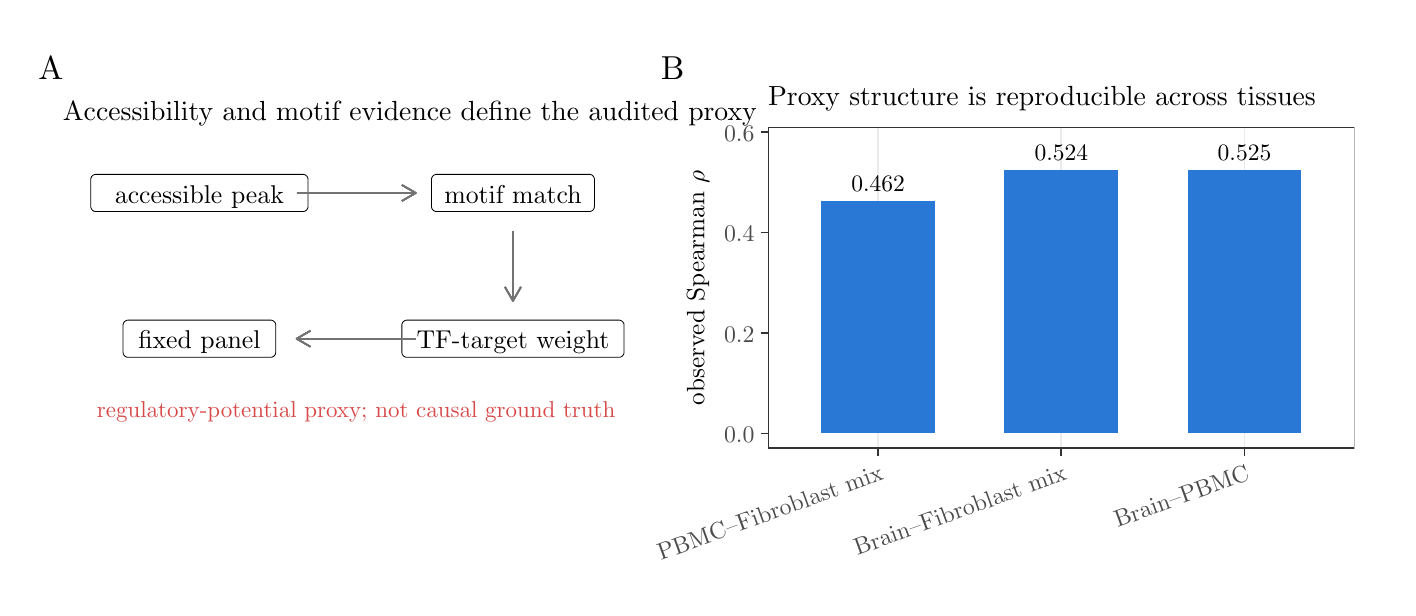
\begin{tikzpicture}[x=1pt,y=1pt]
\definecolor{fillColor}{RGB}{255,255,255}
\path[use as bounding box,fill=fillColor,fill opacity=0.00] (0,0) rectangle (491.44,202.36);
\begin{scope}
\path[clip] (  0.00,  0.00) rectangle (491.44,202.36);
\definecolor{drawColor}{RGB}{255,255,255}
\definecolor{fillColor}{RGB}{255,255,255}

\path[draw=drawColor,line width= 0.6pt,line join=round,line cap=round,fill=fillColor] ( -0.00, -0.00) rectangle (491.44,202.36);
\end{scope}
\begin{scope}
\path[clip] (  4.00,  3.00) rectangle (224.64,198.36);

\path[] (  4.00,  3.00) rectangle (224.64,198.36);
\end{scope}
\begin{scope}
\path[clip] (224.64,  3.00) rectangle (485.44,198.36);
\definecolor{drawColor}{RGB}{255,255,255}
\definecolor{fillColor}{RGB}{255,255,255}

\path[draw=drawColor,line width= 0.6pt,line join=round,line cap=round,fill=fillColor] (224.64,  3.00) rectangle (485.44,198.36);
\end{scope}
\begin{scope}
\path[clip] (  0.00,  0.00) rectangle (491.44,202.36);
\definecolor{drawColor}{RGB}{0,0,0}
\definecolor{fillColor}{RGB}{255,255,255}

\path[draw=drawColor,line width= 0.3pt,line join=round,line cap=round,fill=fillColor] ( 24.65,135.91) --
	( 99.45,135.91) --
	( 99.38,135.92) --
	( 99.68,135.93) --
	( 99.97,135.99) --
	(100.25,136.09) --
	(100.50,136.24) --
	(100.73,136.43) --
	(100.93,136.65) --
	(101.09,136.91) --
	(101.21,137.18) --
	(101.28,137.47) --
	(101.30,137.77) --
	(101.30,137.77) --
	(101.30,147.50) --
	(101.30,147.50) --
	(101.28,147.79) --
	(101.21,148.08) --
	(101.09,148.36) --
	(100.93,148.61) --
	(100.73,148.83) --
	(100.50,149.02) --
	(100.25,149.17) --
	( 99.97,149.28) --
	( 99.68,149.33) --
	( 99.45,149.35) --
	( 24.65,149.35) --
	( 24.87,149.33) --
	( 24.58,149.35) --
	( 24.28,149.31) --
	( 23.99,149.23) --
	( 23.73,149.10) --
	( 23.48,148.93) --
	( 23.27,148.73) --
	( 23.09,148.49) --
	( 22.95,148.22) --
	( 22.85,147.94) --
	( 22.81,147.65) --
	( 22.80,147.50) --
	( 22.80,137.77) --
	( 22.81,137.91) --
	( 22.81,137.62) --
	( 22.85,137.32) --
	( 22.95,137.04) --
	( 23.09,136.78) --
	( 23.27,136.54) --
	( 23.48,136.33) --
	( 23.73,136.16) --
	( 23.99,136.03) --
	( 24.28,135.95) --
	( 24.58,135.92) --
	cycle;
\end{scope}
\begin{scope}
\path[clip] (  0.00,  0.00) rectangle (491.44,202.36);
\definecolor{drawColor}{RGB}{0,0,0}

\node[text=drawColor,anchor=base,inner sep=0pt, outer sep=0pt, scale=  0.93] at ( 62.05,139.00) {accessible peak};
\end{scope}
\begin{scope}
\path[clip] (  0.00,  0.00) rectangle (491.44,202.36);
\definecolor{drawColor}{RGB}{0,0,0}
\definecolor{fillColor}{RGB}{255,255,255}

\path[draw=drawColor,line width= 0.3pt,line join=round,line cap=round,fill=fillColor] (147.77,135.91) --
	(202.94,135.91) --
	(202.86,135.92) --
	(203.16,135.93) --
	(203.45,135.99) --
	(203.73,136.09) --
	(203.99,136.24) --
	(204.22,136.43) --
	(204.42,136.65) --
	(204.58,136.91) --
	(204.69,137.18) --
	(204.76,137.47) --
	(204.79,137.77) --
	(204.79,137.77) --
	(204.79,147.50) --
	(204.79,147.50) --
	(204.76,147.79) --
	(204.69,148.08) --
	(204.58,148.36) --
	(204.42,148.61) --
	(204.22,148.83) --
	(203.99,149.02) --
	(203.73,149.17) --
	(203.45,149.28) --
	(203.16,149.33) --
	(202.94,149.35) --
	(147.77,149.35) --
	(148.00,149.33) --
	(147.70,149.35) --
	(147.40,149.31) --
	(147.12,149.23) --
	(146.85,149.10) --
	(146.60,148.93) --
	(146.39,148.73) --
	(146.21,148.49) --
	(146.07,148.22) --
	(145.98,147.94) --
	(145.93,147.65) --
	(145.92,147.50) --
	(145.92,137.77) --
	(145.93,137.91) --
	(145.93,137.62) --
	(145.98,137.32) --
	(146.07,137.04) --
	(146.21,136.78) --
	(146.39,136.54) --
	(146.60,136.33) --
	(146.85,136.16) --
	(147.12,136.03) --
	(147.40,135.95) --
	(147.70,135.92) --
	cycle;
\end{scope}
\begin{scope}
\path[clip] (  0.00,  0.00) rectangle (491.44,202.36);
\definecolor{drawColor}{RGB}{0,0,0}

\node[text=drawColor,anchor=base,inner sep=0pt, outer sep=0pt, scale=  0.93] at (175.36,139.00) {motif match};
\end{scope}
\begin{scope}
\path[clip] (  0.00,  0.00) rectangle (491.44,202.36);
\definecolor{drawColor}{RGB}{0,0,0}
\definecolor{fillColor}{RGB}{255,255,255}

\path[draw=drawColor,line width= 0.3pt,line join=round,line cap=round,fill=fillColor] (137.06, 83.25) --
	(213.65, 83.25) --
	(213.58, 83.25) --
	(213.88, 83.26) --
	(214.17, 83.32) --
	(214.45, 83.43) --
	(214.70, 83.57) --
	(214.93, 83.76) --
	(215.13, 83.99) --
	(215.29, 84.24) --
	(215.41, 84.51) --
	(215.48, 84.80) --
	(215.50, 85.10) --
	(215.50, 85.10) --
	(215.50, 94.83) --
	(215.50, 94.83) --
	(215.48, 95.13) --
	(215.41, 95.42) --
	(215.29, 95.69) --
	(215.13, 95.94) --
	(214.93, 96.16) --
	(214.70, 96.35) --
	(214.45, 96.50) --
	(214.17, 96.61) --
	(213.88, 96.67) --
	(213.65, 96.68) --
	(137.06, 96.68) --
	(137.28, 96.67) --
	(136.98, 96.68) --
	(136.69, 96.64) --
	(136.40, 96.56) --
	(136.13, 96.43) --
	(135.89, 96.26) --
	(135.67, 96.06) --
	(135.49, 95.82) --
	(135.35, 95.56) --
	(135.26, 95.27) --
	(135.21, 94.98) --
	(135.21, 94.83) --
	(135.21, 85.10) --
	(135.21, 85.25) --
	(135.21, 84.95) --
	(135.26, 84.65) --
	(135.35, 84.37) --
	(135.49, 84.11) --
	(135.67, 83.87) --
	(135.89, 83.66) --
	(136.13, 83.49) --
	(136.40, 83.37) --
	(136.69, 83.28) --
	(136.98, 83.25) --
	cycle;
\end{scope}
\begin{scope}
\path[clip] (  0.00,  0.00) rectangle (491.44,202.36);
\definecolor{drawColor}{RGB}{0,0,0}

\node[text=drawColor,anchor=base,inner sep=0pt, outer sep=0pt, scale=  0.93] at (175.36, 86.33) {TF-target weight};
\end{scope}
\begin{scope}
\path[clip] (  0.00,  0.00) rectangle (491.44,202.36);
\definecolor{drawColor}{RGB}{0,0,0}
\definecolor{fillColor}{RGB}{255,255,255}

\path[draw=drawColor,line width= 0.3pt,line join=round,line cap=round,fill=fillColor] ( 36.32, 83.25) --
	( 87.79, 83.25) --
	( 87.71, 83.25) --
	( 88.01, 83.26) --
	( 88.30, 83.32) --
	( 88.58, 83.43) --
	( 88.84, 83.57) --
	( 89.07, 83.76) --
	( 89.27, 83.99) --
	( 89.43, 84.24) --
	( 89.54, 84.51) --
	( 89.61, 84.80) --
	( 89.64, 85.10) --
	( 89.64, 85.10) --
	( 89.64, 94.83) --
	( 89.64, 94.83) --
	( 89.61, 95.13) --
	( 89.54, 95.42) --
	( 89.43, 95.69) --
	( 89.27, 95.94) --
	( 89.07, 96.16) --
	( 88.84, 96.35) --
	( 88.58, 96.50) --
	( 88.30, 96.61) --
	( 88.01, 96.67) --
	( 87.79, 96.68) --
	( 36.32, 96.68) --
	( 36.54, 96.67) --
	( 36.24, 96.68) --
	( 35.95, 96.64) --
	( 35.66, 96.56) --
	( 35.39, 96.43) --
	( 35.14, 96.26) --
	( 34.93, 96.06) --
	( 34.75, 95.82) --
	( 34.61, 95.56) --
	( 34.52, 95.27) --
	( 34.47, 94.98) --
	( 34.46, 94.83) --
	( 34.46, 85.10) --
	( 34.47, 85.25) --
	( 34.47, 84.95) --
	( 34.52, 84.65) --
	( 34.61, 84.37) --
	( 34.75, 84.11) --
	( 34.93, 83.87) --
	( 35.14, 83.66) --
	( 35.39, 83.49) --
	( 35.66, 83.37) --
	( 35.95, 83.28) --
	( 36.24, 83.25) --
	cycle;
\end{scope}
\begin{scope}
\path[clip] (  0.00,  0.00) rectangle (491.44,202.36);
\definecolor{drawColor}{RGB}{0,0,0}

\node[text=drawColor,anchor=base,inner sep=0pt, outer sep=0pt, scale=  0.93] at ( 62.05, 86.33) {fixed panel};
\end{scope}
\begin{scope}
\path[clip] (  0.00,  0.00) rectangle (491.44,202.36);
\definecolor{drawColor}{gray}{0.45}

\path[draw=drawColor,line width= 0.6pt,line join=round] ( 97.18,142.63) -- (140.23,142.63);

\path[draw=drawColor,line width= 0.6pt,line join=round] (135.22,139.74) --
	(140.23,142.63) --
	(135.22,145.52);

\path[draw=drawColor,line width= 0.6pt,line join=round] ( 97.18,142.63) -- (140.23,142.63);

\path[draw=drawColor,line width= 0.6pt,line join=round] (135.22,139.74) --
	(140.23,142.63) --
	(135.22,145.52);

\path[draw=drawColor,line width= 0.6pt,line join=round] ( 97.18,142.63) -- (140.23,142.63);

\path[draw=drawColor,line width= 0.6pt,line join=round] (135.22,139.74) --
	(140.23,142.63) --
	(135.22,145.52);

\path[draw=drawColor,line width= 0.6pt,line join=round] ( 97.18,142.63) -- (140.23,142.63);

\path[draw=drawColor,line width= 0.6pt,line join=round] (135.22,139.74) --
	(140.23,142.63) --
	(135.22,145.52);

\path[draw=drawColor,line width= 0.6pt,line join=round] (175.36,128.94) -- (175.36,103.66);

\path[draw=drawColor,line width= 0.6pt,line join=round] (172.46,108.66) --
	(175.36,103.66) --
	(178.25,108.66);

\path[draw=drawColor,line width= 0.6pt,line join=round] (175.36,128.94) -- (175.36,103.66);

\path[draw=drawColor,line width= 0.6pt,line join=round] (172.46,108.66) --
	(175.36,103.66) --
	(178.25,108.66);

\path[draw=drawColor,line width= 0.6pt,line join=round] (175.36,128.94) -- (175.36,103.66);

\path[draw=drawColor,line width= 0.6pt,line join=round] (172.46,108.66) --
	(175.36,103.66) --
	(178.25,108.66);

\path[draw=drawColor,line width= 0.6pt,line join=round] (175.36,128.94) -- (175.36,103.66);

\path[draw=drawColor,line width= 0.6pt,line join=round] (172.46,108.66) --
	(175.36,103.66) --
	(178.25,108.66);

\path[draw=drawColor,line width= 0.6pt,line join=round] (140.23, 89.96) -- ( 97.18, 89.96);

\path[draw=drawColor,line width= 0.6pt,line join=round] (102.18, 92.85) --
	( 97.18, 89.96) --
	(102.18, 87.07);

\path[draw=drawColor,line width= 0.6pt,line join=round] (140.23, 89.96) -- ( 97.18, 89.96);

\path[draw=drawColor,line width= 0.6pt,line join=round] (102.18, 92.85) --
	( 97.18, 89.96) --
	(102.18, 87.07);

\path[draw=drawColor,line width= 0.6pt,line join=round] (140.23, 89.96) -- ( 97.18, 89.96);

\path[draw=drawColor,line width= 0.6pt,line join=round] (102.18, 92.85) --
	( 97.18, 89.96) --
	(102.18, 87.07);

\path[draw=drawColor,line width= 0.6pt,line join=round] (140.23, 89.96) -- ( 97.18, 89.96);

\path[draw=drawColor,line width= 0.6pt,line join=round] (102.18, 92.85) --
	( 97.18, 89.96) --
	(102.18, 87.07);
\definecolor{drawColor}{RGB}{216,74,74}

\node[text=drawColor,anchor=base,inner sep=0pt, outer sep=0pt, scale=  0.83] at (118.70, 61.45) {regulatory-potential proxy; not causal ground truth};
\end{scope}
\begin{scope}
\path[clip] (  0.00,  0.00) rectangle (491.44,202.36);
\definecolor{drawColor}{RGB}{0,0,0}

\node[text=drawColor,anchor=base west,inner sep=0pt, outer sep=0pt, scale=  1.00] at ( 12.76,168.77) {Accessibility and motif evidence define the audited proxy};
\end{scope}
\begin{scope}
\path[clip] (  0.00,  0.00) rectangle (491.44,202.36);
\definecolor{drawColor}{RGB}{0,0,0}

\node[text=drawColor,anchor=base,inner sep=0pt, outer sep=0pt, scale=  1.20] at (  8.38,183.53) {A};
\end{scope}
\begin{scope}
\path[clip] (267.56, 50.46) rectangle (479.44,166.33);
\definecolor{fillColor}{RGB}{255,255,255}

\path[fill=fillColor] (267.56, 50.46) rectangle (479.44,166.33);
\definecolor{drawColor}{gray}{0.92}

\path[draw=drawColor,line width= 0.6pt,line join=round] (307.29, 50.46) --
	(307.29,166.33);

\path[draw=drawColor,line width= 0.6pt,line join=round] (373.50, 50.46) --
	(373.50,166.33);

\path[draw=drawColor,line width= 0.6pt,line join=round] (439.71, 50.46) --
	(439.71,166.33);
\definecolor{fillColor}{RGB}{42,120,214}

\path[fill=fillColor] (419.18, 55.73) rectangle (460.23,151.05);

\path[fill=fillColor] (352.97, 55.73) rectangle (394.02,150.99);

\path[fill=fillColor] (286.76, 55.73) rectangle (327.81,139.69);
\definecolor{drawColor}{RGB}{0,0,0}

\node[text=drawColor,anchor=base,inner sep=0pt, outer sep=0pt, scale=  0.85] at (439.71,154.38) {0.525};

\node[text=drawColor,anchor=base,inner sep=0pt, outer sep=0pt, scale=  0.85] at (373.50,154.31) {0.524};

\node[text=drawColor,anchor=base,inner sep=0pt, outer sep=0pt, scale=  0.85] at (307.29,143.02) {0.462};
\definecolor{drawColor}{gray}{0.20}

\path[draw=drawColor,line width= 0.6pt,line join=round,line cap=round] (267.56, 50.46) rectangle (479.44,166.33);
\end{scope}
\begin{scope}
\path[clip] (  0.00,  0.00) rectangle (491.44,202.36);
\definecolor{drawColor}{gray}{0.30}

\node[text=drawColor,anchor=base east,inner sep=0pt, outer sep=0pt, scale=  0.86] at (262.61, 52.36) {0.0};

\node[text=drawColor,anchor=base east,inner sep=0pt, outer sep=0pt, scale=  0.86] at (262.61, 88.68) {0.2};

\node[text=drawColor,anchor=base east,inner sep=0pt, outer sep=0pt, scale=  0.86] at (262.61,125.01) {0.4};

\node[text=drawColor,anchor=base east,inner sep=0pt, outer sep=0pt, scale=  0.86] at (262.61,161.33) {0.6};
\end{scope}
\begin{scope}
\path[clip] (  0.00,  0.00) rectangle (491.44,202.36);
\definecolor{drawColor}{gray}{0.20}

\path[draw=drawColor,line width= 0.6pt,line join=round] (264.81, 55.73) --
	(267.56, 55.73);

\path[draw=drawColor,line width= 0.6pt,line join=round] (264.81, 92.05) --
	(267.56, 92.05);

\path[draw=drawColor,line width= 0.6pt,line join=round] (264.81,128.37) --
	(267.56,128.37);

\path[draw=drawColor,line width= 0.6pt,line join=round] (264.81,164.70) --
	(267.56,164.70);
\end{scope}
\begin{scope}
\path[clip] (  0.00,  0.00) rectangle (491.44,202.36);
\definecolor{drawColor}{gray}{0.20}

\path[draw=drawColor,line width= 0.6pt,line join=round] (307.29, 47.71) --
	(307.29, 50.46);

\path[draw=drawColor,line width= 0.6pt,line join=round] (373.50, 47.71) --
	(373.50, 50.46);

\path[draw=drawColor,line width= 0.6pt,line join=round] (439.71, 47.71) --
	(439.71, 50.46);
\end{scope}
\begin{scope}
\path[clip] (  0.00,  0.00) rectangle (491.44,202.36);
\definecolor{drawColor}{gray}{0.30}

\node[text=drawColor,rotate= 20.00,anchor=base east,inner sep=0pt, outer sep=0pt, scale=  0.86] at (309.59, 39.18) {PBMC--Fibroblast mix};

\node[text=drawColor,rotate= 20.00,anchor=base east,inner sep=0pt, outer sep=0pt, scale=  0.86] at (375.80, 39.18) {Brain--Fibroblast mix};

\node[text=drawColor,rotate= 20.00,anchor=base east,inner sep=0pt, outer sep=0pt, scale=  0.86] at (442.01, 39.18) {Brain--PBMC};
\end{scope}
\begin{scope}
\path[clip] (  0.00,  0.00) rectangle (491.44,202.36);
\definecolor{drawColor}{RGB}{0,0,0}

\node[text=drawColor,rotate= 90.00,anchor=base,inner sep=0pt, outer sep=0pt, scale=  0.91] at (244.50,108.40) {observed Spearman $\rho$};
\end{scope}
\begin{scope}
\path[clip] (  0.00,  0.00) rectangle (491.44,202.36);
\definecolor{drawColor}{RGB}{0,0,0}

\node[text=drawColor,anchor=base west,inner sep=0pt, outer sep=0pt, scale=  1.00] at (267.56,174.27) {Proxy structure is reproducible across tissues};
\end{scope}
\begin{scope}
\path[clip] (  0.00,  0.00) rectangle (491.44,202.36);
\definecolor{drawColor}{RGB}{0,0,0}

\node[text=drawColor,anchor=base,inner sep=0pt, outer sep=0pt, scale=  1.20] at (233.02,183.53) {B};
\end{scope}
\end{tikzpicture}
